\documentclass[11pt]{article}
\usepackage[utf8]{inputenc}
\usepackage{amssymb}
\usepackage[left=1.5in,right=1.5in,top=1.5in,bottom=1.5in]{geometry}
\usepackage{graphicx}
\usepackage{fancyhdr}
\usepackage[hyphens]{url}
\usepackage[hyperfootnotes=false]{hyperref}
\usepackage[font=small,labelfont=bf]{caption}
\usepackage{svg}
\usepackage{caption}
\usepackage{subcaption}
\usepackage[noadjust]{cite} % to cite in ranges
\usepackage{titlesec}

\title{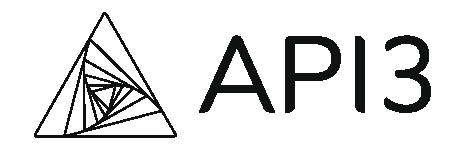
\includegraphics[width=0.7\textwidth]{fig/api3/api3} \\ Oracle Extractable Value (OEV)\\ through Order Flow Auctions
}
\author{Jacob Greene, Ashar Shahid, Burak Benligiray, Heikki Vänttinen}
\date{\hyperref[sec:versions]{v1.0.0} \\ \medskip \href{https://api3.org}{api3.org}}

% no paragraph indents
\setlength\parindent{0pt}
% vertical paragraph spacing
\setlength{\parskip}{1em}
% add dot after section number
\titlelabel{\thetitle.\quad}

\pagestyle{fancy}
\fancyhf{}
\lhead{\small Oracle Extractable Value (OEV) through Order Flow Auctions}
\rhead{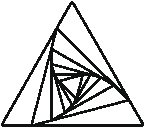
\includegraphics[height=7mm]{fig/api3/api3-solo}}
\fancyfoot[C]{\thepage}

\begin{document}

\pagenumbering{gobble}

\maketitle

%~~~~~~~~~~~~~~~~~~~~~~~~~~~~~~~~~~~~~~~~~~~~~~~~~~~~~~~~~~~~~~~~~~~
\section{Introduction}

While API3 has been building decentralised APIs delivering data to blockchain applications with quantifiable security through service coverage~\cite{api3}, the expectations from oracle services have evolved with the rise of MEV~\cite{flashbots-explore}.
MEV stands for ``maximal extractable value", and is a hidden fee imposed on blockchain users by more strategic third parties extracting value from their transactions.
Stakeholders of most DeFi applications now demand that the MEV extracted from them be minimised, yet existing application designs are predominantly unaware of MEV and thus have forfeited their ability to prevent this value loss.
These design decisions leave most of the MEV to block producers, who capture it by hosting blockspace auctions.
A blockspace auction occurs whenever an MEV opportunity presents itself, and \textit{searchers} bid for the right to have their transaction ordered within that block in a way that allows them to extract value.
This is usually done in the form of probabilistic gas auctions~\cite{Daian:2019}, unless there are off-chain solutions for block producers on that network such as the one popularised by Flashbots for Ethereum~\cite{flashbots-boost}.
{\let\thefootnote\relax\footnote{{We thank Hamza Khan, Torgin Mackinga, Nicolas Laurent and Daniele Pinna for reviewing an earlier version of this paper.}}}

A subset of MEV is related to the way oracles are currently designed, and can be termed ``oracle extractable value" (OEV).
For dApps that rely on oracles, any update to the data feed, or the lack thereof, can create opportunities for OEV such as frontrunning, arbitrage and liquidations.
The value loss caused by OEV has made it difficult for developers to build certain types of dApps, e.g., due to profitability issues for liquidity providers (LPs) that hinder growth on platforms such as Synthetix~\cite{sip-37} and GMX~\cite{kip-17}.
dApps and their users are unable to completely prevent this on their end because they have no control over transactions generated by the oracle, showing a necessity for changes to be implemented within the oracle protocol.

API3 is uniquely poised to provide a solution by auctioning off meta-transactions that are cryptographically signed by first-party oracles, which can be used by third parties to update the data feed in a tamper-proof way.
The entity who is granted access to update the data feed would naturally be guaranteed first rights to any OEV opportunities that come directly before or after the update.
Granting this access at the oracle protocol layer means searchers would no longer have to participate in blockspace auctions for OEV opportunities, and can instead participate in an auction held by the oracle that sends the majority of the value back to the dApp where it was generated.
The dApps would now be in the role of the auction host rather than the block producers, putting them in control of the value they are creating by using data feeds.
This allows them to direct this value towards more productive means that grow their network, creating a crucial role for API3 to facilitate this auction process on behalf of the dApp.

Auctioning the right to request updates as a sidecar to the existing function of the oracle internalises OEV while maintaining security guarantees, as the underlying service is not subjected to additional disruption and latency.
As a side-effect, granularity is improved by incentivising highly specialised actors to provide a more insightful method of determining when to update the on-chain datapoint.

\begin{figure}
	\centering
	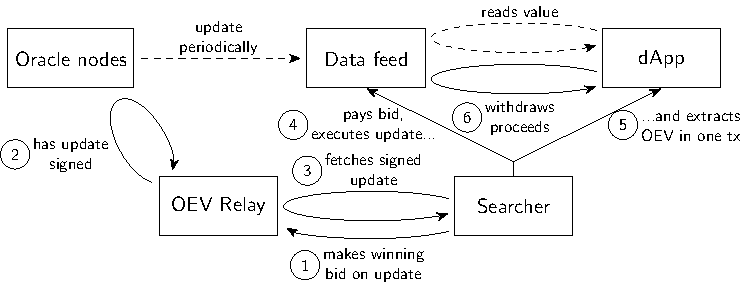
\includegraphics{fig/teaser/teaser}
	\caption{The overview of the order flow auction-based OEV solution.
		Follow the numbered steps for the whole process.
		The dashed arrows represent traditional data feed interactions, which are not mutually exclusive with the proposed solution.}
	\label{fig:teaser}
\end{figure}

See Figure~\ref{fig:teaser} for an overview of the order flow auction that facilitates OEV extraction and distribution, which operates alongside the oracle service that updates the data feed based on deviation thresholds.
The OEV Relay facilitates the auction by intermediating between the searchers and the oracle nodes, using reputation scores and unconditional bids~\cite{flashbots-centralization-2} to prevent searcher misbehaviour.
OEV proceeds are distributed to the dApp that generated the value within the data feed update transaction.
This improves on existing oracle solutions by maximising value capture for the dApp and its users while delivering a higher quality of data, driving demand for data feeds and associated services such as data feed service coverage by API3.

%~~~~~~~~~~~~~~~~~~~~~~~~~~~~~~~~~~~~~~~~~~~~~~~~~~~~~~~~~~~~~~~~~~~
\section{MEV and Oracles}

dApps use oracles to determine the spot price of their supported assets.
This means that changes in the datapoint supplied by oracles lead directly to changes in the state of the markets on these dApps, usually accompanied by a third party extracting value.
There are a few different general types of OEV that can occur as a direct result of these state changes: frontrunning, arbitrage, and liquidations.
The value being extracted must come from somewhere, and in the case of OEV, it is from the liquidity providers on dApps using data feeds.
dApps demand lower deviation thresholds to prevent the losses resulting from OEV, putting a constant pressure on the operational costs of maintaining data feeds.
This leaves the oracle and the dApp struggling to find sustainable profitability, while they leak value to more strategic parties.

\subsection{Frontrunning}

Frontrunning and arbitrage are known as \textit{toxic flow} for derivative protocols because these transactions lead solely to losses for their LPs without providing any meaningful benefits. 
Large data feed customers such as Synthetix have outlined the issue frontrunning poses for LP profitability in proposal~\cite{sip-37}.
By sending their transactions blindly to the public mempool, oracles are publishing the future price of that asset for any dApp using the data feed.
This allows searchers the time to bid for their own transaction to be ordered directly before the oracle transaction, so that they can make a guaranteed profit on the direction of the move.
LPs on these platforms must take the opposite of every trade against the underlying price, and therefore are forced to incur these losses.
Synthetix made progress in limiting this by adding a confirmation period for trades within their protocol, although this was a blow to the user experience and revenue generated.
For the oracle to prevent frontrunning, it would have to use a product such as Flashbots Protect~\cite{flashbots-protect}, which affects the latency and security of the data feed.

\subsection{Arbitrage}

Arbitrage is referenced in both Synthetix~\cite{sip-198} and GMX~\cite{kip-17} proposals, and is also caused by a lack of granularity resulting from deviation threshold-based rules.
If the data feed is showing a stale price relative to another venue, searchers will compete to trade against that price because they can immediately sell it on the other venue for profit.
This results in a constant barrage of unprofitable trades that dApp LPs are again forced to accept, adding to the losses.
As seen in SIP-198~\cite{sip-198}, these issues forced Synthetix to introduce Uniswap TWAP oracles~\cite{uniswap} as a requirement alongside Chainlink to determine pricing of their assets.
This was not a complete fix, as TWAP oracles, by definition, provide a stale price and present an additional barrier for asset-listing.

\subsection{Liquidations}

Liquidations are a necessary function of lending protocols, but the approach to both incentivise and execute them is inefficient, often resulting in value loss for users and difficulties listing assets.

\subsubsection{Borrowers}

dApps pay out a portion of the collateral being liquidated as a part of their security model, but it could be argued that they are overpaying for this while underpaying other important stakeholders, such as their users.
In 2022 to date, over \$300M of collateral was liquidated from lending protocols on Ethereum mainnet, paying out a lower bounds estimate of \$15M in OEV as incentives~\cite{dune-liquidations}.
Lending protocols such as Euler Finance~\cite{euler} are attempting to address this by retaining some of the OEV for borrowers using a form of a Dutch auction that allows the incentive (discount percentage) to vary.
By placing the dApps or their borrowers as auction hosts for liquidation opportunities, more of this value can now be distributed back to them, although adding latency with an on-chain auction introduces other tradeoffs.

\subsubsection{Lenders}

Currently, most oracle designs decide when to update the on-chain datapoint by comparing it to the off-chain datapoint, and updating it whenever the deviation between the two crosses a predetermined threshold.
This causes situations when there is a liquidation that needs to occur, but the on-chain datapoint does not reflect the current asset price, and thus does not allow for the liquidation.
This results in lenders potentially receiving less collateral back than they otherwise would have with a more granular data feed.
The inefficiency also means that data feeds are extremely expensive to operate, forcing protocols like Euler to rely on TWAP oracles as a method of listing assets~\cite{euler}.
This introduces new challenges because having sufficiently liquid Uniswap pools on each network is not an easy requirement to meet, and TWAPs provide stale data, presenting more possible hindrances to lender profitability.

%~~~~~~~~~~~~~~~~~~~~~~~~~~~~~~~~~~~~~~~~~~~~~~~~~~~~~~~~~~~~~~~~~~~
\section{Order Flow (OF) Auctions}

Any intent from an actor to change the state of the blockchain is an order, and a collection or stream of these is called order flow (OF).
Actors who are not highly skilled in MEV themselves need a way to retain the value currently being extracted from their orders.
OF auctions provide a way to accomplish this by mimicking blockspace auctions, and offering the right to extract MEV to third parties, but position the actor generating the order as the auction host rather than block producers.
This auction process must be as credibly-neutral as possible to avoid the risks that distributing OF to a few exclusive parties would pose to the decentralisation of the network~\cite{flashbots-centralization-1}.

MEV related to frontrunning of transactions was mitigated by users replacing the standard RPC with a private communication channel to entities that promise not to gossip the transactions or extract any MEV, while still including them in a block~\cite{flashbots-protect}.
It is impossible to prevent the portion of MEV that is available through backrunning (transactions occurring directly after data feed updates) because it includes liquidations and arbitrage, which are necessary for the system.
Therefore, this MEV should be efficiently extracted and returned to the actor creating it.
A competitive market for private channels has led to OF auctions being implemented, which offer the unavoidable portion of MEV back to actors as an incentive to send transactions to that channel.
Provided that the auction process is well-designed, this puts the actor into a position of power over the MEV they generate. 

For applications that propagate significant amounts of MEV-generating transactions such as an oracle, the easiest technical solution would be to offer all of their OF to a single dominant searcher.
Centralisation of OF in this way could lead to rent extraction, poor user experience, and few entities gaining undue influence over the network.
This has driven researchers to encourage highly competitive auction processes from developers of these systems~\cite{flashbots-centralization-2}.
Since most of these actors cannot be expected to host decentralised OF auctions for themselves, entities like Rook~\cite{rook} provide this as a service alongside transaction inclusion.

\begin{figure}
	\centering
	\begin{subfigure}{0.49\textwidth}
		\centering
		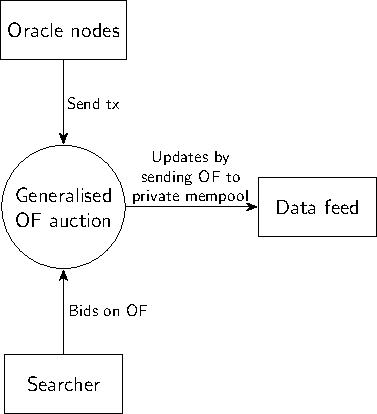
\includegraphics{fig/of-auction/of-auction-a}
		\caption{Generalised OF auction}
		\label{fig:of-auction-a}
	\end{subfigure}
	\hfill
	\begin{subfigure}{0.49\textwidth}
		\centering
		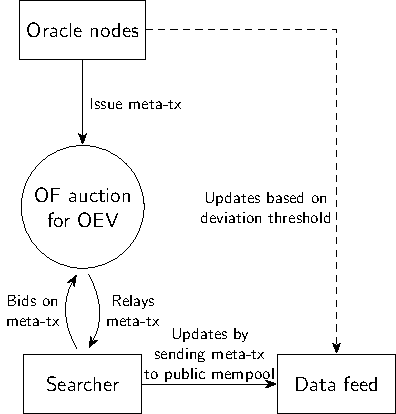
\includegraphics{fig/of-auction/of-auction-b}
		\caption{OF auction specialised for OEV}
		\label{fig:of-auction-b}
	\end{subfigure}
	\caption{A comparison of \textbf{(a)} generalised OF auctions and \textbf{(b)} proposed OF auctions specialised for OEV.}
	\label{fig:of-auction}
\end{figure}

While there are multiple entities building generalised MEV solutions that an oracle could send their transactions to~\cite{flashbots-suave,rook}, existing OF auction designs introduce latency that decreases the reliability and security of data feeds.
Instead of being able to send transactions directly to block producers, there is now an auction round that must conclude beforehand (see Figure~\ref{fig:of-auction-a}).
Every transaction would suffer from added latency because the oracle will not have any insight into whether they generate any OEV or not, and must send all of their transactions to the auction.
Oracles also have to consider that private communication channels may experience downtime because they will not be as decentralised as the public mempool, which adds even more potential latency to transactions.
These risks would result in many of the data feed updates being unnecessarily delayed, which may cause added value loss for the LPs, making these OF auctions an unacceptable disruption of the oracle service.

\subsection{Benefits of an OF Auction Specialised for OEV}

An oracle can avoid the risks associated with generalised OF auctions by developing a mechanism that generates transactions upon request, alongside the existing design propagating transactions to the public mempool based on deviation thresholds  (see Figure~\ref{fig:of-auction-b}).
This allows for a fallback alongside the auction that maintains the security guarantees of the data feed, and allows the oracle to provide service coverage for them.
Another benefit of allowing searchers to request data feed updates is that it increases the granularity of the data. This means that instead of just minimising MEV extraction from users, OEV OF auctions take this a step further and seek to maximise user revenue and experience.
Requesting OF is possible because it is always desirable for an oracle to update their data feed—they are only constrained by gas costs in doing so.
These constraints create a perfect scenario to outsource the updating of data feeds to searchers who will not have to rely on deviation thresholds as a trigger, and instead have insight into the dApp's specific needs.
A much more efficient system can be designed where data feeds are updated exactly when the dApp requires a more recent datapoint, instead of the current more ineffective and wasteful approach.

\subsection{Effects of OF Auctions Specialised for OEV on MEV}

OEV auctions will not prevent \textbf{frontrunning}, but instead aim minimise the value loss.
A first-price-sealed-bid auction process~\cite{fpsba}, under perfect competition, should result in the value extracted from frontrunning OEV data feeds approaching the cost of blockspace for executing the opportunity.
This means that LPs are compensating searchers the minimal amount they need to for gas and transaction execution of data feed updates, in the form of frontrunning profits.
Outsourcing the role of performing data feed updates to searchers provides economic guarantees of a more performant oracle designed to maximise revenue for LPs.

More granular data prevents much of the toxic flow presented to the protocol LPs from \textbf{arbitrage}, and maximises the retention of any that still exists through the auction.
Improving the profitability of LPs should provide users with deeper liquidity and better pricing, allowing for more assets to be listed, which benefits the entire network.

A more accurate data feed protects lender capital with timely \textbf{liquidations}, and the OEV auction maximises capital returned to liquidated borrowers.
The increased granularity driven by requesting OF gives lenders more capital protection, which should allow them to list more assets and create more value.
In addition, due to the fact that oracles operate off-chain, they can implement sealed-bid auctions that would not be possible for protocols that operate on-chain, allowing for potentially higher value retention for liquidated borrowers. 

%~~~~~~~~~~~~~~~~~~~~~~~~~~~~~~~~~~~~~~~~~~~~~~~~~~~~~~~~~~~~~~~~~~~
\section{Requesting OF from First-party Oracles}

Searchers can initiate data feed updates by requesting a \textit{meta-transaction} that is cryptographically signed by the first-party oracles.
The meta-transaction can be used by third parties to update data feeds in a tamper-proof way~\cite{airnode-sign}.
Searchers will transition from watching the public mempool for OEV opportunities, to querying an API managed by the oracle that returns the current off-chain price for each data feed.
Once searchers identify a new datapoint that would trigger an OEV opportunity, they can place a bid for it, and upon the conclusion of each auction round, a meta-transaction is returned to the respective winning bidder.
Searchers must include the meta-transaction internally within their OEV transaction.
Data providers sign the meta-transaction along with the public key of the winning bidder to ensure that the transaction cannot be frontrun.
This creates a mechanism that will not be dependent on private communication channels or other special deals with block producers, which most OF auctions would usually require.
The bid amount will also be included in the signature as a way of enforcing payment when the data feed is updated.
Hosting the OEV auction off-chain also reduces gas costs for searchers and regular users of the network.
Networks without off-chain MEV auctions like this suffer from the bloat of probabilistic gas auctions within the public mempool that increase costs for everyone~\cite{Daian:2019}.

Added benefits of the oracle developing and managing their own OF auction is that it:
\begin{itemize}
	\item Removes dependencies on outside services;
	\item Allows the OEV to be shared between stakeholders without compensating middlemen;
	\item Empowers OEV internalisation across all blockchains where data feeds are integrated.
\end{itemize}

%~~~~~~~~~~~~~~~~~~~~~~~~~~~~~~~~~~~~~~~~~~~~~~~~~~~~~~~~~~~~~~~~~~~
\section{OEV Relay}

\begin{figure}
	\centering
	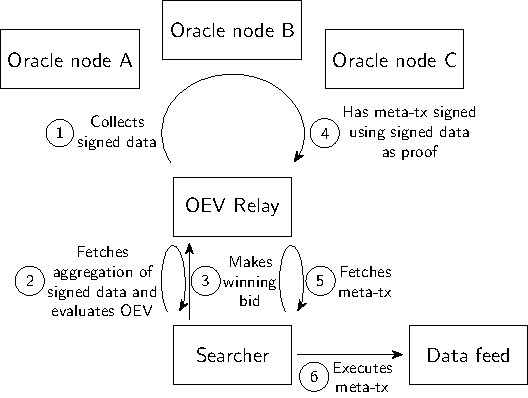
\includegraphics{fig/oev-relay/oev-relay}
	\caption{An auction facilitated by the OEV Relay.
		Follow the numbered steps for the auction process.
		The OEV Relay provides searchers with a united auction interface so that they do not have to interact with individual oracle nodes, and shields the individual oracle nodes from misbehaving searchers.}
	\label{fig:oev-relay}
\end{figure}

OEV auctions will use another popular concept from Flashbots, a third party API that implements denial of service (DOS) protection for the auction hosts~\cite{flashbots-boost-relays}, which in this case will be the first-party oracles.
This API is termed the ``OEV Relay", and will compensate first-party oracles for winning bids, and be responsible for curating the network of searchers.
Another role that the OEV Relay plays is to maximise the auction proceeds without requiring coordination between data providers.
These aspects help to maintain the simplicity and security of the first-party oracle software (Airnode~\cite{airnode}), which is crucial for gaining adoption from data providers.
See Figure~\ref{fig:oev-relay} for a visualisation of the OEV Relay and how it interacts with searchers and the oracle nodes.

OF auctions are significantly different from blockspace auctions because their hosts do not possess control over transaction inclusion, as they are not block producers.
This means that the OEV Relay does not have the ability to guarantee that searchers will follow through on agreements made with it.
Searchers may propose bids that they never intend to pay out in order to censor others, or they may overbid for an opportunity and be unable to pay.
This creates the necessity for methods of disincentivizing such undesirable actions.
When designing these disincentivization methods, it is important to understand that any added uncertainty or impact to the experience of the searchers is expected to result in lower bid amounts.

The following are the proposed methods to enforce agreements between searchers and the OEV Relay:
\begin{itemize}
	\item \textbf{Reputation scores:} Pioneered by Rook, reputation scoring is based on monitoring searcher activity after auctions conclude~\cite{rook-reputation}.
	The OEV Relay can do this by watching for events from the data feed contract, and reducing reputation scores of searchers who fail to update data feeds that they agreed to.
	This concept uses the incentives of future revenue to prevent misbehaviour, but does not allow for a permissionless auction.
	\item \textbf{Unconditional bids:} The OEV Relay could also require unconditional bids by forcing searchers to commit to payment before utilizing the meta-transaction.
	This will lead to lower auction proceeds because searchers have to factor in the risk of not being able to capitalize on the OEV opportunity in time.
	So a good system may be requiring that only part of the bid be unconditional.
\end{itemize}

Both reputation scoring and unconditional bids provide tradeoffs for searchers, making it important to experiment with combinations of them to arrive at a relay that maximises bid amounts while maintaining decentralisation.

Another difference between OF auctions and blockspace auctions is that the latter has a bidding period defined by a network's block times.
Implementing auction times that are close to average block times on the respective network should increase value capture for the OEV Relay, but auctions must never conclude quicker than block inclusion.
A requirement of the OEV Relay is that the auction process should be conducted significantly quicker than the underlying oracle service performs data feed updates.
Searchers will be racing to update the data feed before deviation thresholds are triggered, as this would lead to updates being sent to the public mempool and forfeiting any OEV.

The runner of this relay will be unable to tamper with any of the data because it is signed by the providers.
It is not possible for the relay to steal OEV opportunities because it does not require searchers to expose their own transactions beforehand.
The worst exploit the relay can perform is to censor bids and extract the OEV themselves.
It should be noted that oracles can already do this by sending their transactions to private mempools bundled with OEV capturing transactions, but as the oracle operation decentralises further, so can the relay.
The data providers can be distributed a portion of the auction proceeds to cover their costs and enhance security of the operation.
By providing an efficient way for applications to distribute a portion of the value they create to the data providers, we more closely align the oracle and the applications using their data.
Properly incentivising data provision to blockchains will lead to an abundant network of providers competing to offer the best service, in turn leading to novel applications being built on top of it.

%~~~~~~~~~~~~~~~~~~~~~~~~~~~~~~~~~~~~~~~~~~~~~~~~~~~~~~~~~~~~~~~~~~~
\section{Accurate OEV Distribution}

There is a tradeoff between being able to accurately distribute OEV to the corresponding application that it was generated on, and multiple applications being able to share OEV-generated data feed updates.
For example, if two derivative applications share a data feed for ETH/USD, changes in the state of this datapoint are likely to trigger OEV opportunities on both applications in the same auction period.
Due to the fact that these applications both read from the same datapoint on-chain, there is no way to trustlessly isolate the auctions for each application, so searchers must place one bid for both opportunities, making it intractable to distribute the proceeds accurately.

\begin{figure}
	\centering
	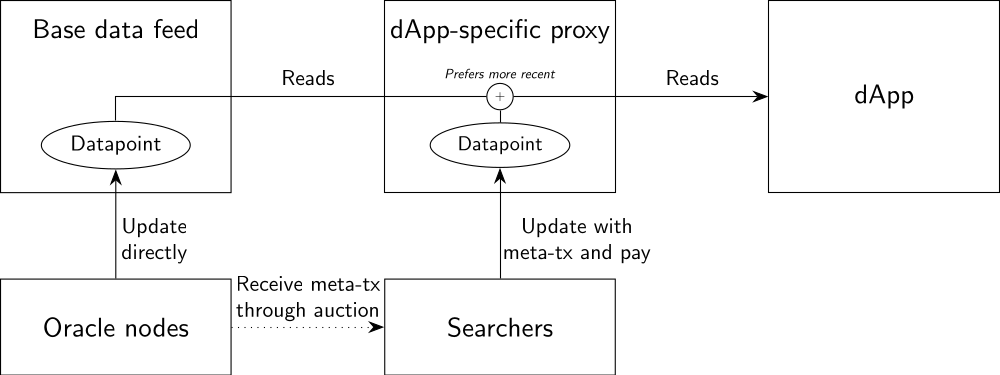
\includegraphics{fig/oev-distribution/oev-distribution}
	\caption{dApp-specific data feed proxies enable dApp-specific OEV updates, which allows accurate accumulation of respective auction proceeds.
		The proxies prefer deviation threshold-based updates if they are more recent, which creates an automatic fallback mechanism when OEV-based updates are disrupted.}
	\label{fig:oev-distribution}
\end{figure}

A solution to accurately and immediately distribute the OEV is to create data feeds for each application.
Application-specific data feeds will be an abstraction on top of base data feeds that are updated by the oracle when deviation thresholds are crossed.
Application-specific data feeds share data from the base data feed that they are mapped to, but will each also have their own respective datapoint (see Figure~\ref{fig:oev-distribution}).
The oracle can now host auctions for the application-specific data feeds, allowing searchers to bid for each application's OEV distinctly, and in a trustless manner.
This is done without forcing the oracle to take on higher operational costs or change its service by maintaining the mapping to base data feeds, which allows it to still update every application-specific feed with a single transaction.

Accurate OEV distribution via application-specific data feeds should produce a significantly better user experience, while imposing little overhead for the DAO operating it.
Applications can integrate with these data feeds and begin retaining their OEV without any development needed on their end.

\subsection{Integrating a dApp to OEV data feeds}

A dApp is integrated to an OEV-enabled data feed through the following steps:

\begin{enumerate}
	\item Application registers to an OEV feed through a marketplace UI or smart contract function call, and specifies the address that they would like the OEV sent to.
	\item Once registered, their application-specific data feed contract is deployed. The application can read from it as they would any existing oracle solution.
	\item The contract deployment will trigger an event that the OEV relay sees, and it will now process requests for signatures to that data feed.
	\item Searchers begin placing bids for signed data, and the OEV is distributed to the respective application during the data feed update transaction.
\end{enumerate}

It should be noted that if applications were willing to share the auction proceeds in a way that is not accurate, they could then benefit from the positive effects of sharing OEV updates.
This would mean that when OEV is generated on one application but not the other, they both get to share the updated datapoint and granularity that comes from it without incurring any extra cost.

%~~~~~~~~~~~~~~~~~~~~~~~~~~~~~~~~~~~~~~~~~~~~~~~~~~~~~~~~~~~~~~~~~~~
\section{Conclusion}
\label{sec:conclusion}

Decentralised finance applications have been limited by existing oracle services that allow significant value loss for their users in the form of OEV.
This is caused by constraints for blockspace and sub-optimal mechanisms for updating data feeds.
By developing a new type of OF auction specialised to request data from oracles on demand, OEV data feeds enable a more performant method of providing data by outsourcing updates to highly specialised actors, which aims to maximise value capture for dApps and users.
This will result in improvements to pricing accuracy and, therefore, should generate additional revenue for applications that rely on this data, creating powerful incentives to use OEV data feeds.

\small
\bibliographystyle{ieeetr}
\bibliography{refs}

\normalsize
\appendix
\section{Versions}
\label{sec:versions}
\href{https://github.com/api3dao/oev-litepaper/releases/tag/v1.0.0}{v1.0.0} -- Jacob Greene, Ashar Shahid, Burak Benligiray, Heikki Vänttinen, November 2022.

\section{Disclaimer}
\label{sec:disclaimer}

The writings herein are for information purposes only, and do not constitute financial, legal, or other professional advice of any kind, nor do they commit any authors or any related entities or persons to undertake any described or implied actions.
Any forward-looking statements herein are subject to risks, uncertainties, and assumptions which could prove to be inaccurate and, as a result, such statements could be materially incorrect and readers should not rely upon them.

Neither the authors nor any of their affiliates, nor any of their respective directors, advisors, contractors, employees or representatives make any representations or warranties, express or implied, with respect to any of the material or information contained herein, nor do any of the foregoing assume or otherwise have any responsibility or any obligation or liability whatsoever to any reader, any reader's affiliates, or any of such reader's or such reader's affiliates' respective directors, advisors, contractors, employees or representatives resulting from the use of the information and material contained herein.

\end{document}
